\documentclass[../RASD.tex]{subfiles}
\graphicspath{{\subfix{../assets}}}

\begin{document}

The analysis using Alloy tool aims to formally prove the correctness of the model previously described.
To achieve so, a test to assert the satisfaction of the goals has been made.
In particular the following goals have been tested:
\begin{itemize}
    \item {\textbf{(G1) Have his/her own profile on the application}: for this goal an assertion called \textit{DifferentEmailOrNicknameImpliesDifferentUsers} checks that no user have same e-mail or nickname}
    \item {\textbf{(G2) Participate in a coding tournament}: to satisfy this goal an assertion called \textit{StudentsSubscribedToBattleAlsoSubscribedToTournament} verifies that only a user that is subscribed to the tournament where the battle is being hosted can enroll to that battle.
    The predicate \textit{StudentParticipatesInTournament} shows that some students can subscribe to a tournament where a battle is being hosted.}
    \item {\textbf{(G3) Cooperate with colleagues}: to fulfill this goal some assertions have been made:
    \begin{itemize}
        \item \textit{StudentInGroupAlsoInBattle} checks that a student must be enrolled in a battle to be part of a group
        \item \textit{NoLoneSolution} checks that a solution must be submitted by a group that is participating to such a battle
        \item \textit{GroupSizeIsCorrect} checks that every group is in the size constrain limit of a battle
    \end{itemize}
    Furthermore, a predicate called \textit{StudentCollaborateWithColleagues} shows a student collaborating with a group and the relative solution}
    \item {\textbf{(G4) Review their own performance score}: using the predicate \textit{showStudentSolutions} the model shows all the solutions published by a student in the context of a tournament.
    Given a set of solution is then possible to calculate, using the desired performance metrics, the score of a student(in the context of such a tournament)}
    \item {\textbf{(G5) Organize coding tournaments}: for this goal an assertion called \textit{NoEducatorWithoutTournament} checks that all educators are linked to a tournament.
    The predicate \textit{showEducatorsInTournament} instead shows some educators administering a tournament}
    \item {\textbf{(G6) Run coding battles in their tournaments}: to satisfy this goal an assertion called \textit{BattleOwnerIsEducatorOfTournament} verifies that all the battles inside a tournament have been created by an educator of such a tournament}
    \item {\textbf{(G7) Close an existing coding battle in their tournaments}: using the predicate \textit{showClosedBattle} the model shows an instance were a battle has been closed}
    \item {\textbf{(G8 \& G9) Obtain an automated evaluation over a student solution \& Manually review students submissions}: to fulfill these goals an assertion called \textit{CorrectSolutionScore} checks that all the solutions have an automated score and that the manual score is set if and only if it was needed(manual review score was enabled in the settings of a battle)}
\end{itemize}

\newpage

\subsection{Alloy Code}\label{subsec:alloy_code}
    \lstinputlisting[language=alloy]{../alloy/alloy.als}

\newpage

Here below some predicates generated by the model are shown.
\begin{figure}[h!]
    \centering
    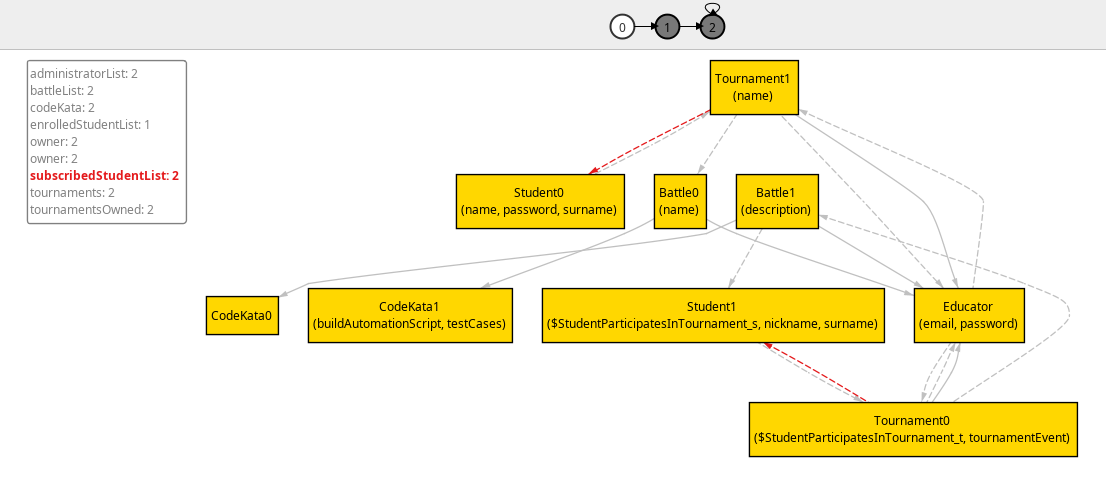
\includegraphics[width=\textwidth]{../assets/section_4/StudentParticipatesInTournament_0.png}
    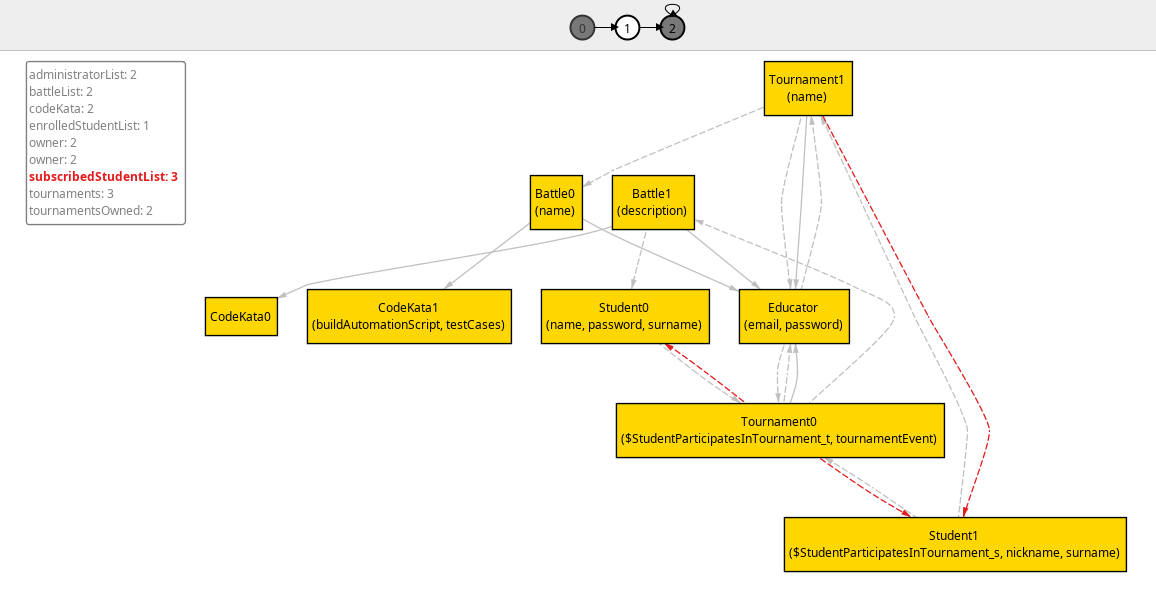
\includegraphics[width=\textwidth]{../assets/section_4/StudentParticipatesInTournament_1.png}
    \caption{Predicate \textit{StudentParticipatesInTournament}.}
    \label{img:alloy_student_participates_in_tournament}
\end{figure}

\newpage

\begin{figure}[h!]
    \centering
    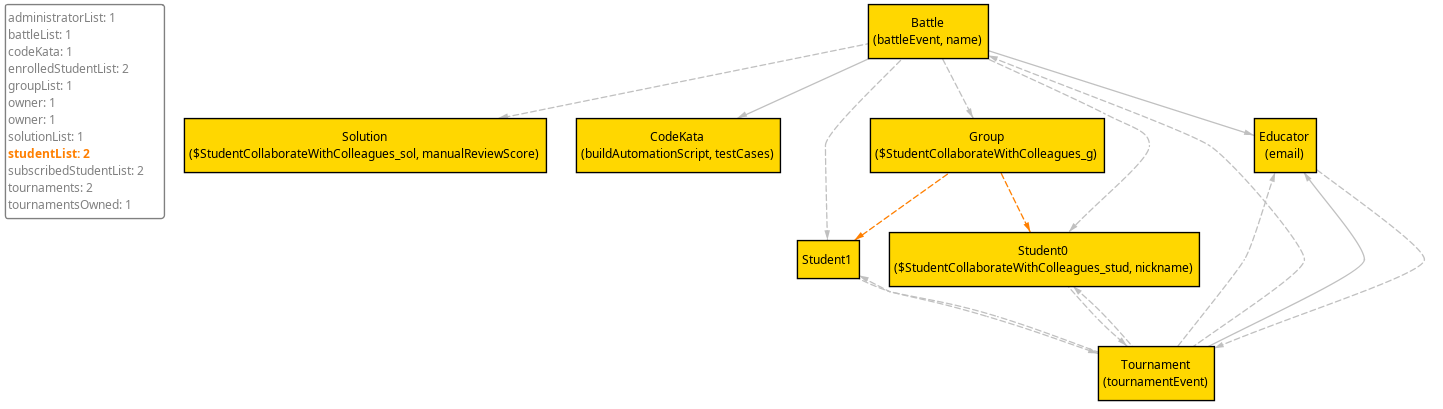
\includegraphics[width=1.2\textwidth, angle=90]{../assets/section_4/StudentCollaborateWithColleagues.png}
    \caption{Predicate \textit{StudentCollaborateWithColleagues}.}
    \label{img:alloy_student_collaborate_with_colleagues}
\end{figure}

\newpage

\begin{figure}[h!]
    \centering
    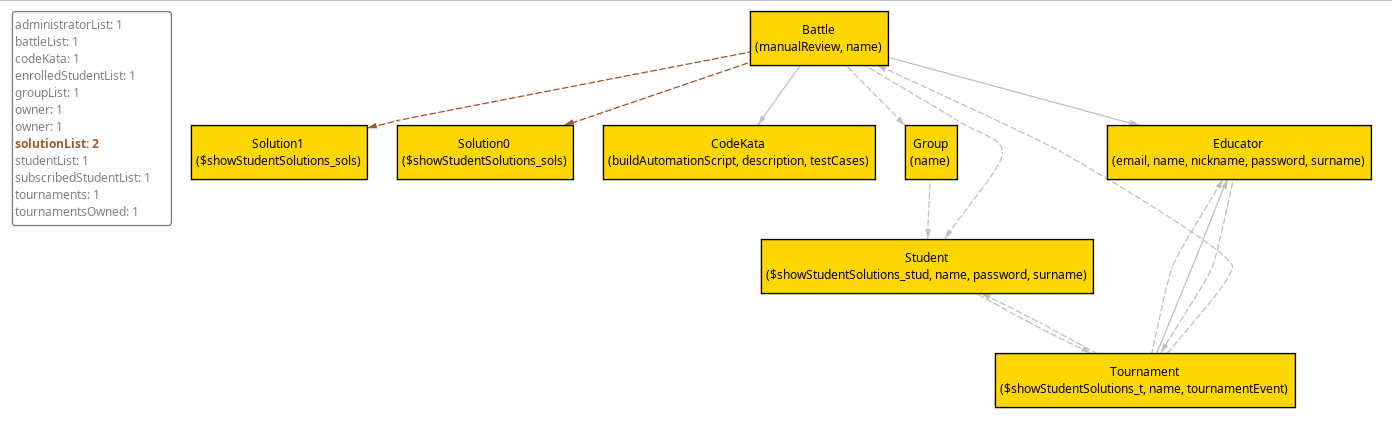
\includegraphics[width=1.2\textwidth, angle=90]{../assets/section_4/showStudentSolutions.png}
    \caption{Predicate \textit{showStudentSolutions}.}
    \label{img:alloy_show_student_solutions}
\end{figure}

\newpage

\begin{figure}[h!]
    \centering
    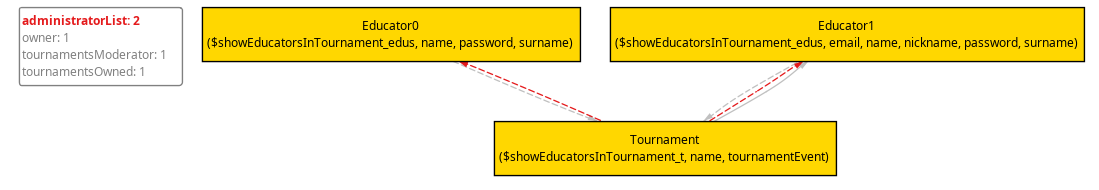
\includegraphics[width=\textwidth]{../assets/section_4/showEducatorsInTournament.png}
    \caption{Predicate \textit{showEducatorsInTournament}.}
    \label{img:alloy_show_educators_in_tournament}
\end{figure}
\newpage

\begin{figure}[h!]
    \centering
    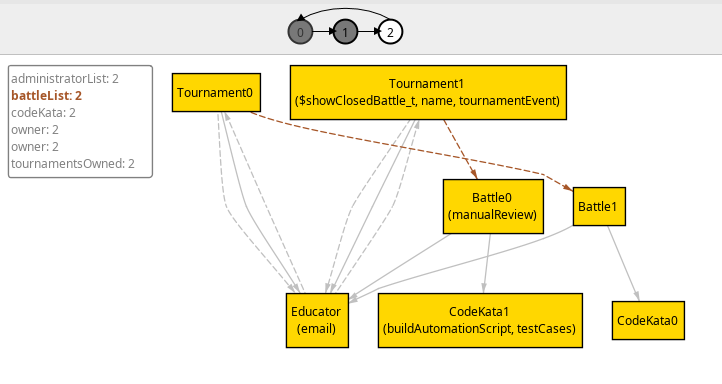
\includegraphics[width=\textwidth]{../assets/section_4/showClosedBattle_0.png}
    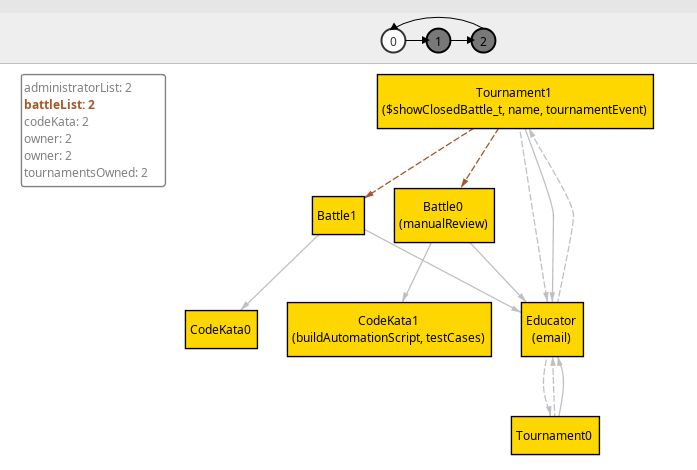
\includegraphics[width=\textwidth]{../assets/section_4/showClosedBattle_1.png}
    \caption{Predicate \textit{showClosedBattle}.}
    \label{img:alloy_show_closed_battle}
\end{figure}

\end{document}